% Created by tikzDevice version 0.7.0 on 2014-07-01 17:48:13
% !TEX encoding = UTF-8 Unicode
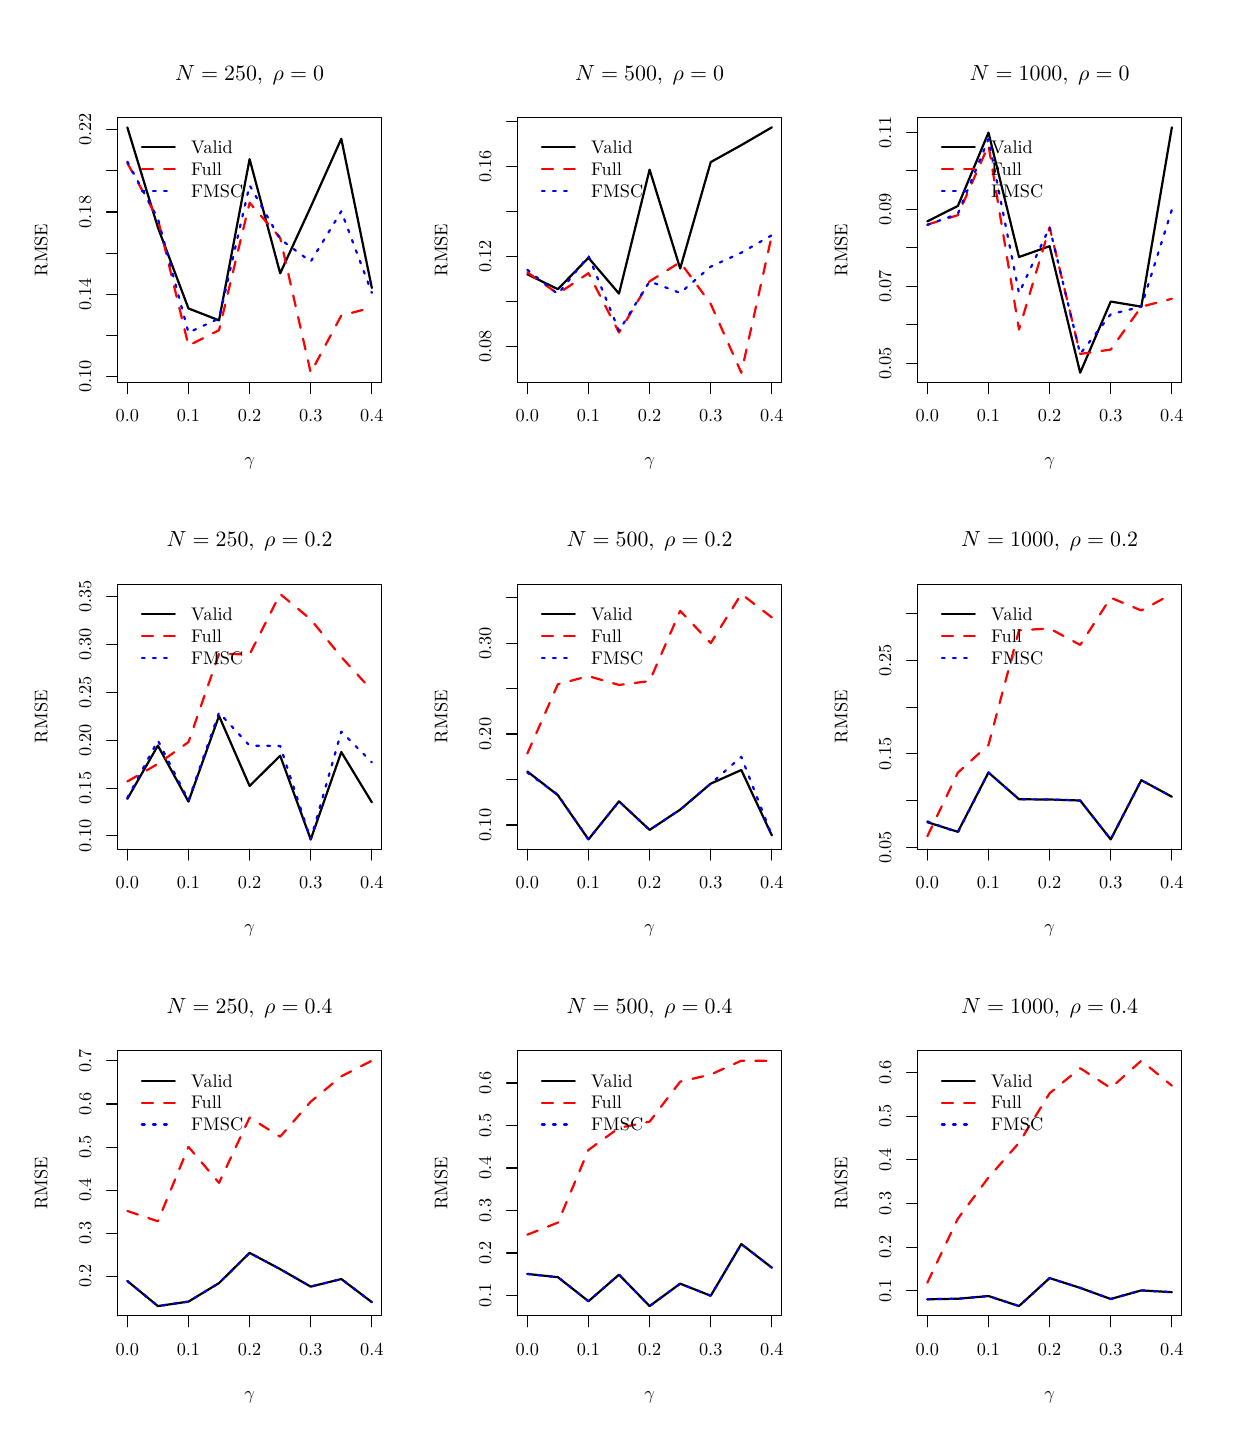
\begin{tikzpicture}[x=1pt,y=1pt]
\definecolor[named]{fillColor}{rgb}{1.00,1.00,1.00}
\path[use as bounding box,fill=fillColor,fill opacity=0.00] (0,0) rectangle (433.62,505.89);
\begin{scope}
\path[clip] ( 32.47,377.65) rectangle (127.91,473.42);
\definecolor[named]{drawColor}{rgb}{0.00,0.00,0.00}

\path[draw=drawColor,line width= 0.8pt,line join=round,line cap=round] ( 36.01,469.87) --
	( 47.05,433.70) --
	( 58.10,404.43) --
	( 69.14,400.13) --
	( 80.19,458.38) --
	( 91.24,417.13) --
	(102.28,441.11) --
	(113.33,465.73) --
	(124.37,411.81);
\end{scope}
\begin{scope}
\path[clip] (  0.00,  0.00) rectangle (433.62,505.89);
\definecolor[named]{drawColor}{rgb}{0.00,0.00,0.00}

\path[draw=drawColor,line width= 0.4pt,line join=round,line cap=round] ( 36.01,377.65) -- (124.37,377.65);

\path[draw=drawColor,line width= 0.4pt,line join=round,line cap=round] ( 36.01,377.65) -- ( 36.01,373.69);

\path[draw=drawColor,line width= 0.4pt,line join=round,line cap=round] ( 58.10,377.65) -- ( 58.10,373.69);

\path[draw=drawColor,line width= 0.4pt,line join=round,line cap=round] ( 80.19,377.65) -- ( 80.19,373.69);

\path[draw=drawColor,line width= 0.4pt,line join=round,line cap=round] (102.28,377.65) -- (102.28,373.69);

\path[draw=drawColor,line width= 0.4pt,line join=round,line cap=round] (124.37,377.65) -- (124.37,373.69);

\node[text=drawColor,anchor=base,inner sep=0pt, outer sep=0pt, scale=  0.66] at ( 36.01,363.40) {0.0};

\node[text=drawColor,anchor=base,inner sep=0pt, outer sep=0pt, scale=  0.66] at ( 58.10,363.40) {0.1};

\node[text=drawColor,anchor=base,inner sep=0pt, outer sep=0pt, scale=  0.66] at ( 80.19,363.40) {0.2};

\node[text=drawColor,anchor=base,inner sep=0pt, outer sep=0pt, scale=  0.66] at (102.28,363.40) {0.3};

\node[text=drawColor,anchor=base,inner sep=0pt, outer sep=0pt, scale=  0.66] at (124.37,363.40) {0.4};

\path[draw=drawColor,line width= 0.4pt,line join=round,line cap=round] ( 32.47,379.75) -- ( 32.47,469.04);

\path[draw=drawColor,line width= 0.4pt,line join=round,line cap=round] ( 32.47,379.75) -- ( 28.51,379.75);

\path[draw=drawColor,line width= 0.4pt,line join=round,line cap=round] ( 32.47,394.63) -- ( 28.51,394.63);

\path[draw=drawColor,line width= 0.4pt,line join=round,line cap=round] ( 32.47,409.51) -- ( 28.51,409.51);

\path[draw=drawColor,line width= 0.4pt,line join=round,line cap=round] ( 32.47,424.40) -- ( 28.51,424.40);

\path[draw=drawColor,line width= 0.4pt,line join=round,line cap=round] ( 32.47,439.28) -- ( 28.51,439.28);

\path[draw=drawColor,line width= 0.4pt,line join=round,line cap=round] ( 32.47,454.16) -- ( 28.51,454.16);

\path[draw=drawColor,line width= 0.4pt,line join=round,line cap=round] ( 32.47,469.04) -- ( 28.51,469.04);

\node[text=drawColor,rotate= 90.00,anchor=base,inner sep=0pt, outer sep=0pt, scale=  0.66] at ( 22.97,379.75) {0.10};

\node[text=drawColor,rotate= 90.00,anchor=base,inner sep=0pt, outer sep=0pt, scale=  0.66] at ( 22.97,409.51) {0.14};

\node[text=drawColor,rotate= 90.00,anchor=base,inner sep=0pt, outer sep=0pt, scale=  0.66] at ( 22.97,439.28) {0.18};

\node[text=drawColor,rotate= 90.00,anchor=base,inner sep=0pt, outer sep=0pt, scale=  0.66] at ( 22.97,469.04) {0.22};

\path[draw=drawColor,line width= 0.4pt,line join=round,line cap=round] ( 32.47,377.65) --
	(127.91,377.65) --
	(127.91,473.42) --
	( 32.47,473.42) --
	( 32.47,377.65);
\end{scope}
\begin{scope}
\path[clip] (  0.00,337.26) rectangle (144.54,505.89);
\definecolor[named]{drawColor}{rgb}{0.00,0.00,0.00}

\node[text=drawColor,anchor=base,inner sep=0pt, outer sep=0pt, scale=  0.79] at ( 80.19,486.92) {\bfseries $N=250, \;\rho=0$};

\node[text=drawColor,anchor=base,inner sep=0pt, outer sep=0pt, scale=  0.66] at ( 80.19,347.56) {$\gamma$};

\node[text=drawColor,rotate= 90.00,anchor=base,inner sep=0pt, outer sep=0pt, scale=  0.66] at (  7.13,425.53) {RMSE};
\end{scope}
\begin{scope}
\path[clip] ( 32.47,377.65) rectangle (127.91,473.42);
\definecolor[named]{drawColor}{rgb}{1.00,0.00,0.00}

\path[draw=drawColor,line width= 0.8pt,dash pattern=on 4pt off 4pt ,line join=round,line cap=round] ( 36.01,456.99) --
	( 47.05,436.71) --
	( 58.10,391.00) --
	( 69.14,396.56) --
	( 80.19,442.61) --
	( 91.24,429.94) --
	(102.28,381.20) --
	(113.33,401.86) --
	(124.37,404.76);
\definecolor[named]{drawColor}{rgb}{0.00,0.00,1.00}

\path[draw=drawColor,line width= 0.8pt,dash pattern=on 1pt off 3pt ,line join=round,line cap=round] ( 36.01,457.47) --
	( 47.05,436.91) --
	( 58.10,395.69) --
	( 69.14,400.79) --
	( 80.19,448.94) --
	( 91.24,429.48) --
	(102.28,421.35) --
	(113.33,439.53) --
	(124.37,410.04);
\definecolor[named]{drawColor}{rgb}{0.00,0.00,0.00}

\path[draw=drawColor,line width= 0.8pt,line join=round,line cap=round] ( 41.28,462.63) -- ( 53.16,462.63);
\definecolor[named]{drawColor}{rgb}{1.00,0.00,0.00}

\path[draw=drawColor,line width= 0.8pt,dash pattern=on 4pt off 4pt ,line join=round,line cap=round] ( 41.28,454.71) -- ( 53.16,454.71);
\definecolor[named]{drawColor}{rgb}{0.00,0.00,1.00}

\path[draw=drawColor,line width= 0.8pt,dash pattern=on 1pt off 3pt ,line join=round,line cap=round] ( 41.28,446.79) -- ( 53.16,446.79);
\definecolor[named]{drawColor}{rgb}{0.00,0.00,0.00}

\node[text=drawColor,anchor=base west,inner sep=0pt, outer sep=0pt, scale=  0.66] at ( 59.10,460.35) {Valid};

\node[text=drawColor,anchor=base west,inner sep=0pt, outer sep=0pt, scale=  0.66] at ( 59.10,452.43) {Full};

\node[text=drawColor,anchor=base west,inner sep=0pt, outer sep=0pt, scale=  0.66] at ( 59.10,444.51) {FMSC};
\end{scope}
\begin{scope}
\path[clip] (177.01,377.65) rectangle (272.45,473.42);
\definecolor[named]{drawColor}{rgb}{0.00,0.00,0.00}

\path[draw=drawColor,line width= 0.8pt,line join=round,line cap=round] (180.55,416.77) --
	(191.59,411.39) --
	(202.64,422.73) --
	(213.68,409.79) --
	(224.73,454.59) --
	(235.78,418.84) --
	(246.82,457.30) --
	(257.87,463.44) --
	(268.91,469.87);
\end{scope}
\begin{scope}
\path[clip] (  0.00,  0.00) rectangle (433.62,505.89);
\definecolor[named]{drawColor}{rgb}{0.00,0.00,0.00}

\path[draw=drawColor,line width= 0.4pt,line join=round,line cap=round] (180.55,377.65) -- (268.91,377.65);

\path[draw=drawColor,line width= 0.4pt,line join=round,line cap=round] (180.55,377.65) -- (180.55,373.69);

\path[draw=drawColor,line width= 0.4pt,line join=round,line cap=round] (202.64,377.65) -- (202.64,373.69);

\path[draw=drawColor,line width= 0.4pt,line join=round,line cap=round] (224.73,377.65) -- (224.73,373.69);

\path[draw=drawColor,line width= 0.4pt,line join=round,line cap=round] (246.82,377.65) -- (246.82,373.69);

\path[draw=drawColor,line width= 0.4pt,line join=round,line cap=round] (268.91,377.65) -- (268.91,373.69);

\node[text=drawColor,anchor=base,inner sep=0pt, outer sep=0pt, scale=  0.66] at (180.55,363.40) {0.0};

\node[text=drawColor,anchor=base,inner sep=0pt, outer sep=0pt, scale=  0.66] at (202.64,363.40) {0.1};

\node[text=drawColor,anchor=base,inner sep=0pt, outer sep=0pt, scale=  0.66] at (224.73,363.40) {0.2};

\node[text=drawColor,anchor=base,inner sep=0pt, outer sep=0pt, scale=  0.66] at (246.82,363.40) {0.3};

\node[text=drawColor,anchor=base,inner sep=0pt, outer sep=0pt, scale=  0.66] at (268.91,363.40) {0.4};

\path[draw=drawColor,line width= 0.4pt,line join=round,line cap=round] (177.01,390.75) -- (177.01,472.12);

\path[draw=drawColor,line width= 0.4pt,line join=round,line cap=round] (177.01,390.75) -- (173.05,390.75);

\path[draw=drawColor,line width= 0.4pt,line join=round,line cap=round] (177.01,407.02) -- (173.05,407.02);

\path[draw=drawColor,line width= 0.4pt,line join=round,line cap=round] (177.01,423.30) -- (173.05,423.30);

\path[draw=drawColor,line width= 0.4pt,line join=round,line cap=round] (177.01,439.57) -- (173.05,439.57);

\path[draw=drawColor,line width= 0.4pt,line join=round,line cap=round] (177.01,455.85) -- (173.05,455.85);

\path[draw=drawColor,line width= 0.4pt,line join=round,line cap=round] (177.01,472.12) -- (173.05,472.12);

\node[text=drawColor,rotate= 90.00,anchor=base,inner sep=0pt, outer sep=0pt, scale=  0.66] at (167.51,390.75) {0.08};

\node[text=drawColor,rotate= 90.00,anchor=base,inner sep=0pt, outer sep=0pt, scale=  0.66] at (167.51,423.30) {0.12};

\node[text=drawColor,rotate= 90.00,anchor=base,inner sep=0pt, outer sep=0pt, scale=  0.66] at (167.51,455.85) {0.16};

\path[draw=drawColor,line width= 0.4pt,line join=round,line cap=round] (177.01,377.65) --
	(272.45,377.65) --
	(272.45,473.42) --
	(177.01,473.42) --
	(177.01,377.65);
\end{scope}
\begin{scope}
\path[clip] (144.54,337.26) rectangle (289.08,505.89);
\definecolor[named]{drawColor}{rgb}{0.00,0.00,0.00}

\node[text=drawColor,anchor=base,inner sep=0pt, outer sep=0pt, scale=  0.79] at (224.73,486.92) {\bfseries $N=500, \;\rho=0$};

\node[text=drawColor,anchor=base,inner sep=0pt, outer sep=0pt, scale=  0.66] at (224.73,347.56) {$\gamma$};

\node[text=drawColor,rotate= 90.00,anchor=base,inner sep=0pt, outer sep=0pt, scale=  0.66] at (151.67,425.53) {RMSE};
\end{scope}
\begin{scope}
\path[clip] (177.01,377.65) rectangle (272.45,473.42);
\definecolor[named]{drawColor}{rgb}{1.00,0.00,0.00}

\path[draw=drawColor,line width= 0.8pt,dash pattern=on 4pt off 4pt ,line join=round,line cap=round] (180.55,417.51) --
	(191.59,409.74) --
	(202.64,417.16) --
	(213.68,395.72) --
	(224.73,414.21) --
	(235.78,421.16) --
	(246.82,406.04) --
	(257.87,381.20) --
	(268.91,430.90);
\definecolor[named]{drawColor}{rgb}{0.00,0.00,1.00}

\path[draw=drawColor,line width= 0.8pt,dash pattern=on 1pt off 3pt ,line join=round,line cap=round] (180.55,418.40) --
	(191.59,409.61) --
	(202.64,423.42) --
	(213.68,396.38) --
	(224.73,414.21) --
	(235.78,410.02) --
	(246.82,419.53) --
	(257.87,424.57) --
	(268.91,430.90);
\definecolor[named]{drawColor}{rgb}{0.00,0.00,0.00}

\path[draw=drawColor,line width= 0.8pt,line join=round,line cap=round] (185.82,462.63) -- (197.70,462.63);
\definecolor[named]{drawColor}{rgb}{1.00,0.00,0.00}

\path[draw=drawColor,line width= 0.8pt,dash pattern=on 4pt off 4pt ,line join=round,line cap=round] (185.82,454.71) -- (197.70,454.71);
\definecolor[named]{drawColor}{rgb}{0.00,0.00,1.00}

\path[draw=drawColor,line width= 0.8pt,dash pattern=on 1pt off 3pt ,line join=round,line cap=round] (185.82,446.79) -- (197.70,446.79);
\definecolor[named]{drawColor}{rgb}{0.00,0.00,0.00}

\node[text=drawColor,anchor=base west,inner sep=0pt, outer sep=0pt, scale=  0.66] at (203.64,460.35) {Valid};

\node[text=drawColor,anchor=base west,inner sep=0pt, outer sep=0pt, scale=  0.66] at (203.64,452.43) {Full};

\node[text=drawColor,anchor=base west,inner sep=0pt, outer sep=0pt, scale=  0.66] at (203.64,444.51) {FMSC};
\end{scope}
\begin{scope}
\path[clip] (321.55,377.65) rectangle (416.99,473.42);
\definecolor[named]{drawColor}{rgb}{0.00,0.00,0.00}

\path[draw=drawColor,line width= 0.8pt,line join=round,line cap=round] (325.09,435.89) --
	(336.13,441.47) --
	(347.18,467.97) --
	(358.22,423.01) --
	(369.27,426.92) --
	(380.32,381.20) --
	(391.36,406.92) --
	(402.41,405.07) --
	(413.45,469.87);
\end{scope}
\begin{scope}
\path[clip] (  0.00,  0.00) rectangle (433.62,505.89);
\definecolor[named]{drawColor}{rgb}{0.00,0.00,0.00}

\path[draw=drawColor,line width= 0.4pt,line join=round,line cap=round] (325.09,377.65) -- (413.45,377.65);

\path[draw=drawColor,line width= 0.4pt,line join=round,line cap=round] (325.09,377.65) -- (325.09,373.69);

\path[draw=drawColor,line width= 0.4pt,line join=round,line cap=round] (347.18,377.65) -- (347.18,373.69);

\path[draw=drawColor,line width= 0.4pt,line join=round,line cap=round] (369.27,377.65) -- (369.27,373.69);

\path[draw=drawColor,line width= 0.4pt,line join=round,line cap=round] (391.36,377.65) -- (391.36,373.69);

\path[draw=drawColor,line width= 0.4pt,line join=round,line cap=round] (413.45,377.65) -- (413.45,373.69);

\node[text=drawColor,anchor=base,inner sep=0pt, outer sep=0pt, scale=  0.66] at (325.09,363.40) {0.0};

\node[text=drawColor,anchor=base,inner sep=0pt, outer sep=0pt, scale=  0.66] at (347.18,363.40) {0.1};

\node[text=drawColor,anchor=base,inner sep=0pt, outer sep=0pt, scale=  0.66] at (369.27,363.40) {0.2};

\node[text=drawColor,anchor=base,inner sep=0pt, outer sep=0pt, scale=  0.66] at (391.36,363.40) {0.3};

\node[text=drawColor,anchor=base,inner sep=0pt, outer sep=0pt, scale=  0.66] at (413.45,363.40) {0.4};

\path[draw=drawColor,line width= 0.4pt,line join=round,line cap=round] (321.55,384.67) -- (321.55,468.02);

\path[draw=drawColor,line width= 0.4pt,line join=round,line cap=round] (321.55,384.67) -- (317.59,384.67);

\path[draw=drawColor,line width= 0.4pt,line join=round,line cap=round] (321.55,398.56) -- (317.59,398.56);

\path[draw=drawColor,line width= 0.4pt,line join=round,line cap=round] (321.55,412.45) -- (317.59,412.45);

\path[draw=drawColor,line width= 0.4pt,line join=round,line cap=round] (321.55,426.34) -- (317.59,426.34);

\path[draw=drawColor,line width= 0.4pt,line join=round,line cap=round] (321.55,440.24) -- (317.59,440.24);

\path[draw=drawColor,line width= 0.4pt,line join=round,line cap=round] (321.55,454.13) -- (317.59,454.13);

\path[draw=drawColor,line width= 0.4pt,line join=round,line cap=round] (321.55,468.02) -- (317.59,468.02);

\node[text=drawColor,rotate= 90.00,anchor=base,inner sep=0pt, outer sep=0pt, scale=  0.66] at (312.05,384.67) {0.05};

\node[text=drawColor,rotate= 90.00,anchor=base,inner sep=0pt, outer sep=0pt, scale=  0.66] at (312.05,412.45) {0.07};

\node[text=drawColor,rotate= 90.00,anchor=base,inner sep=0pt, outer sep=0pt, scale=  0.66] at (312.05,440.24) {0.09};

\node[text=drawColor,rotate= 90.00,anchor=base,inner sep=0pt, outer sep=0pt, scale=  0.66] at (312.05,468.02) {0.11};

\path[draw=drawColor,line width= 0.4pt,line join=round,line cap=round] (321.55,377.65) --
	(416.99,377.65) --
	(416.99,473.42) --
	(321.55,473.42) --
	(321.55,377.65);
\end{scope}
\begin{scope}
\path[clip] (289.08,337.26) rectangle (433.62,505.89);
\definecolor[named]{drawColor}{rgb}{0.00,0.00,0.00}

\node[text=drawColor,anchor=base,inner sep=0pt, outer sep=0pt, scale=  0.79] at (369.27,486.92) {\bfseries $N=1000, \;\rho=0$};

\node[text=drawColor,anchor=base,inner sep=0pt, outer sep=0pt, scale=  0.66] at (369.27,347.56) {$\gamma$};

\node[text=drawColor,rotate= 90.00,anchor=base,inner sep=0pt, outer sep=0pt, scale=  0.66] at (296.21,425.53) {RMSE};
\end{scope}
\begin{scope}
\path[clip] (321.55,377.65) rectangle (416.99,473.42);
\definecolor[named]{drawColor}{rgb}{1.00,0.00,0.00}

\path[draw=drawColor,line width= 0.8pt,dash pattern=on 4pt off 4pt ,line join=round,line cap=round] (325.09,434.70) --
	(336.13,438.14) --
	(347.18,463.39) --
	(358.22,396.80) --
	(369.27,433.73) --
	(380.32,387.98) --
	(391.36,389.57) --
	(402.41,405.04) --
	(413.45,407.93);
\definecolor[named]{drawColor}{rgb}{0.00,0.00,1.00}

\path[draw=drawColor,line width= 0.8pt,dash pattern=on 1pt off 3pt ,line join=round,line cap=round] (325.09,434.61) --
	(336.13,438.62) --
	(347.18,465.63) --
	(358.22,409.98) --
	(369.27,433.73) --
	(380.32,387.98) --
	(391.36,402.35) --
	(402.41,405.04) --
	(413.45,440.13);
\definecolor[named]{drawColor}{rgb}{0.00,0.00,0.00}

\path[draw=drawColor,line width= 0.8pt,line join=round,line cap=round] (330.36,462.63) -- (342.24,462.63);
\definecolor[named]{drawColor}{rgb}{1.00,0.00,0.00}

\path[draw=drawColor,line width= 0.8pt,dash pattern=on 4pt off 4pt ,line join=round,line cap=round] (330.36,454.71) -- (342.24,454.71);
\definecolor[named]{drawColor}{rgb}{0.00,0.00,1.00}

\path[draw=drawColor,line width= 0.8pt,dash pattern=on 1pt off 3pt ,line join=round,line cap=round] (330.36,446.79) -- (342.24,446.79);
\definecolor[named]{drawColor}{rgb}{0.00,0.00,0.00}

\node[text=drawColor,anchor=base west,inner sep=0pt, outer sep=0pt, scale=  0.66] at (348.18,460.35) {Valid};

\node[text=drawColor,anchor=base west,inner sep=0pt, outer sep=0pt, scale=  0.66] at (348.18,452.43) {Full};

\node[text=drawColor,anchor=base west,inner sep=0pt, outer sep=0pt, scale=  0.66] at (348.18,444.51) {FMSC};
\end{scope}
\begin{scope}
\path[clip] ( 32.47,209.02) rectangle (127.91,304.79);
\definecolor[named]{drawColor}{rgb}{0.00,0.00,0.00}

\path[draw=drawColor,line width= 0.8pt,line join=round,line cap=round] ( 36.01,227.20) --
	( 47.05,246.46) --
	( 58.10,226.23) --
	( 69.14,257.19) --
	( 80.19,231.88) --
	( 91.24,242.80) --
	(102.28,212.57) --
	(113.33,244.14) --
	(124.37,225.96);
\end{scope}
\begin{scope}
\path[clip] (  0.00,  0.00) rectangle (433.62,505.89);
\definecolor[named]{drawColor}{rgb}{0.00,0.00,0.00}

\path[draw=drawColor,line width= 0.4pt,line join=round,line cap=round] ( 36.01,209.02) -- (124.37,209.02);

\path[draw=drawColor,line width= 0.4pt,line join=round,line cap=round] ( 36.01,209.02) -- ( 36.01,205.06);

\path[draw=drawColor,line width= 0.4pt,line join=round,line cap=round] ( 58.10,209.02) -- ( 58.10,205.06);

\path[draw=drawColor,line width= 0.4pt,line join=round,line cap=round] ( 80.19,209.02) -- ( 80.19,205.06);

\path[draw=drawColor,line width= 0.4pt,line join=round,line cap=round] (102.28,209.02) -- (102.28,205.06);

\path[draw=drawColor,line width= 0.4pt,line join=round,line cap=round] (124.37,209.02) -- (124.37,205.06);

\node[text=drawColor,anchor=base,inner sep=0pt, outer sep=0pt, scale=  0.66] at ( 36.01,194.77) {0.0};

\node[text=drawColor,anchor=base,inner sep=0pt, outer sep=0pt, scale=  0.66] at ( 58.10,194.77) {0.1};

\node[text=drawColor,anchor=base,inner sep=0pt, outer sep=0pt, scale=  0.66] at ( 80.19,194.77) {0.2};

\node[text=drawColor,anchor=base,inner sep=0pt, outer sep=0pt, scale=  0.66] at (102.28,194.77) {0.3};

\node[text=drawColor,anchor=base,inner sep=0pt, outer sep=0pt, scale=  0.66] at (124.37,194.77) {0.4};

\path[draw=drawColor,line width= 0.4pt,line join=round,line cap=round] ( 32.47,213.84) -- ( 32.47,300.27);

\path[draw=drawColor,line width= 0.4pt,line join=round,line cap=round] ( 32.47,213.84) -- ( 28.51,213.84);

\path[draw=drawColor,line width= 0.4pt,line join=round,line cap=round] ( 32.47,231.12) -- ( 28.51,231.12);

\path[draw=drawColor,line width= 0.4pt,line join=round,line cap=round] ( 32.47,248.41) -- ( 28.51,248.41);

\path[draw=drawColor,line width= 0.4pt,line join=round,line cap=round] ( 32.47,265.70) -- ( 28.51,265.70);

\path[draw=drawColor,line width= 0.4pt,line join=round,line cap=round] ( 32.47,282.98) -- ( 28.51,282.98);

\path[draw=drawColor,line width= 0.4pt,line join=round,line cap=round] ( 32.47,300.27) -- ( 28.51,300.27);

\node[text=drawColor,rotate= 90.00,anchor=base,inner sep=0pt, outer sep=0pt, scale=  0.66] at ( 22.97,213.84) {0.10};

\node[text=drawColor,rotate= 90.00,anchor=base,inner sep=0pt, outer sep=0pt, scale=  0.66] at ( 22.97,231.12) {0.15};

\node[text=drawColor,rotate= 90.00,anchor=base,inner sep=0pt, outer sep=0pt, scale=  0.66] at ( 22.97,248.41) {0.20};

\node[text=drawColor,rotate= 90.00,anchor=base,inner sep=0pt, outer sep=0pt, scale=  0.66] at ( 22.97,265.70) {0.25};

\node[text=drawColor,rotate= 90.00,anchor=base,inner sep=0pt, outer sep=0pt, scale=  0.66] at ( 22.97,282.98) {0.30};

\node[text=drawColor,rotate= 90.00,anchor=base,inner sep=0pt, outer sep=0pt, scale=  0.66] at ( 22.97,300.27) {0.35};

\path[draw=drawColor,line width= 0.4pt,line join=round,line cap=round] ( 32.47,209.02) --
	(127.91,209.02) --
	(127.91,304.79) --
	( 32.47,304.79) --
	( 32.47,209.02);
\end{scope}
\begin{scope}
\path[clip] (  0.00,168.63) rectangle (144.54,337.26);
\definecolor[named]{drawColor}{rgb}{0.00,0.00,0.00}

\node[text=drawColor,anchor=base,inner sep=0pt, outer sep=0pt, scale=  0.79] at ( 80.19,318.29) {\bfseries $N=250, \;\rho=0.2$};

\node[text=drawColor,anchor=base,inner sep=0pt, outer sep=0pt, scale=  0.66] at ( 80.19,178.93) {$\gamma$};

\node[text=drawColor,rotate= 90.00,anchor=base,inner sep=0pt, outer sep=0pt, scale=  0.66] at (  7.13,256.90) {RMSE};
\end{scope}
\begin{scope}
\path[clip] ( 32.47,209.02) rectangle (127.91,304.79);
\definecolor[named]{drawColor}{rgb}{1.00,0.00,0.00}

\path[draw=drawColor,line width= 0.8pt,dash pattern=on 4pt off 4pt ,line join=round,line cap=round] ( 36.01,233.50) --
	( 47.05,239.84) --
	( 58.10,247.74) --
	( 69.14,279.63) --
	( 80.19,279.42) --
	( 91.24,301.24) --
	(102.28,292.07) --
	(113.33,278.45) --
	(124.37,266.47);
\definecolor[named]{drawColor}{rgb}{0.00,0.00,1.00}

\path[draw=drawColor,line width= 0.8pt,dash pattern=on 1pt off 3pt ,line join=round,line cap=round] ( 36.01,227.56) --
	( 47.05,248.29) --
	( 58.10,226.66) --
	( 69.14,258.38) --
	( 80.19,246.46) --
	( 91.24,246.32) --
	(102.28,212.57) --
	(113.33,251.51) --
	(124.37,240.42);
\definecolor[named]{drawColor}{rgb}{0.00,0.00,0.00}

\path[draw=drawColor,line width= 0.8pt,line join=round,line cap=round] ( 41.28,294.00) -- ( 53.16,294.00);
\definecolor[named]{drawColor}{rgb}{1.00,0.00,0.00}

\path[draw=drawColor,line width= 0.8pt,dash pattern=on 4pt off 4pt ,line join=round,line cap=round] ( 41.28,286.08) -- ( 53.16,286.08);
\definecolor[named]{drawColor}{rgb}{0.00,0.00,1.00}

\path[draw=drawColor,line width= 0.8pt,dash pattern=on 1pt off 3pt ,line join=round,line cap=round] ( 41.28,278.16) -- ( 53.16,278.16);
\definecolor[named]{drawColor}{rgb}{0.00,0.00,0.00}

\node[text=drawColor,anchor=base west,inner sep=0pt, outer sep=0pt, scale=  0.66] at ( 59.10,291.72) {Valid};

\node[text=drawColor,anchor=base west,inner sep=0pt, outer sep=0pt, scale=  0.66] at ( 59.10,283.80) {Full};

\node[text=drawColor,anchor=base west,inner sep=0pt, outer sep=0pt, scale=  0.66] at ( 59.10,275.88) {FMSC};
\end{scope}
\begin{scope}
\path[clip] (177.01,209.02) rectangle (272.45,304.79);
\definecolor[named]{drawColor}{rgb}{0.00,0.00,0.00}

\path[draw=drawColor,line width= 0.8pt,line join=round,line cap=round] (180.55,237.11) --
	(191.59,228.54) --
	(202.64,212.57) --
	(213.68,226.32) --
	(224.73,216.00) --
	(235.78,223.32) --
	(246.82,232.72) --
	(257.87,237.65) --
	(268.91,214.00);
\end{scope}
\begin{scope}
\path[clip] (  0.00,  0.00) rectangle (433.62,505.89);
\definecolor[named]{drawColor}{rgb}{0.00,0.00,0.00}

\path[draw=drawColor,line width= 0.4pt,line join=round,line cap=round] (180.55,209.02) -- (268.91,209.02);

\path[draw=drawColor,line width= 0.4pt,line join=round,line cap=round] (180.55,209.02) -- (180.55,205.06);

\path[draw=drawColor,line width= 0.4pt,line join=round,line cap=round] (202.64,209.02) -- (202.64,205.06);

\path[draw=drawColor,line width= 0.4pt,line join=round,line cap=round] (224.73,209.02) -- (224.73,205.06);

\path[draw=drawColor,line width= 0.4pt,line join=round,line cap=round] (246.82,209.02) -- (246.82,205.06);

\path[draw=drawColor,line width= 0.4pt,line join=round,line cap=round] (268.91,209.02) -- (268.91,205.06);

\node[text=drawColor,anchor=base,inner sep=0pt, outer sep=0pt, scale=  0.66] at (180.55,194.77) {0.0};

\node[text=drawColor,anchor=base,inner sep=0pt, outer sep=0pt, scale=  0.66] at (202.64,194.77) {0.1};

\node[text=drawColor,anchor=base,inner sep=0pt, outer sep=0pt, scale=  0.66] at (224.73,194.77) {0.2};

\node[text=drawColor,anchor=base,inner sep=0pt, outer sep=0pt, scale=  0.66] at (246.82,194.77) {0.3};

\node[text=drawColor,anchor=base,inner sep=0pt, outer sep=0pt, scale=  0.66] at (268.91,194.77) {0.4};

\path[draw=drawColor,line width= 0.4pt,line join=round,line cap=round] (177.01,217.78) -- (177.01,299.92);

\path[draw=drawColor,line width= 0.4pt,line join=round,line cap=round] (177.01,217.78) -- (173.05,217.78);

\path[draw=drawColor,line width= 0.4pt,line join=round,line cap=round] (177.01,234.21) -- (173.05,234.21);

\path[draw=drawColor,line width= 0.4pt,line join=round,line cap=round] (177.01,250.64) -- (173.05,250.64);

\path[draw=drawColor,line width= 0.4pt,line join=round,line cap=round] (177.01,267.07) -- (173.05,267.07);

\path[draw=drawColor,line width= 0.4pt,line join=round,line cap=round] (177.01,283.50) -- (173.05,283.50);

\path[draw=drawColor,line width= 0.4pt,line join=round,line cap=round] (177.01,299.92) -- (173.05,299.92);

\node[text=drawColor,rotate= 90.00,anchor=base,inner sep=0pt, outer sep=0pt, scale=  0.66] at (167.51,217.78) {0.10};

\node[text=drawColor,rotate= 90.00,anchor=base,inner sep=0pt, outer sep=0pt, scale=  0.66] at (167.51,250.64) {0.20};

\node[text=drawColor,rotate= 90.00,anchor=base,inner sep=0pt, outer sep=0pt, scale=  0.66] at (167.51,283.50) {0.30};

\path[draw=drawColor,line width= 0.4pt,line join=round,line cap=round] (177.01,209.02) --
	(272.45,209.02) --
	(272.45,304.79) --
	(177.01,304.79) --
	(177.01,209.02);
\end{scope}
\begin{scope}
\path[clip] (144.54,168.63) rectangle (289.08,337.26);
\definecolor[named]{drawColor}{rgb}{0.00,0.00,0.00}

\node[text=drawColor,anchor=base,inner sep=0pt, outer sep=0pt, scale=  0.79] at (224.73,318.29) {\bfseries $N=500, \;\rho=0.2$};

\node[text=drawColor,anchor=base,inner sep=0pt, outer sep=0pt, scale=  0.66] at (224.73,178.93) {$\gamma$};

\node[text=drawColor,rotate= 90.00,anchor=base,inner sep=0pt, outer sep=0pt, scale=  0.66] at (151.67,256.90) {RMSE};
\end{scope}
\begin{scope}
\path[clip] (177.01,209.02) rectangle (272.45,304.79);
\definecolor[named]{drawColor}{rgb}{1.00,0.00,0.00}

\path[draw=drawColor,line width= 0.8pt,dash pattern=on 4pt off 4pt ,line join=round,line cap=round] (180.55,243.61) --
	(191.59,268.63) --
	(202.64,271.56) --
	(213.68,268.38) --
	(224.73,269.78) --
	(235.78,295.16) --
	(246.82,283.49) --
	(257.87,301.24) --
	(268.91,292.78);
\definecolor[named]{drawColor}{rgb}{0.00,0.00,1.00}

\path[draw=drawColor,line width= 0.8pt,dash pattern=on 1pt off 3pt ,line join=round,line cap=round] (180.55,236.71) --
	(191.59,228.69) --
	(202.64,212.57) --
	(213.68,226.32) --
	(224.73,216.00) --
	(235.78,223.32) --
	(246.82,232.72) --
	(257.87,242.41) --
	(268.91,214.00);
\definecolor[named]{drawColor}{rgb}{0.00,0.00,0.00}

\path[draw=drawColor,line width= 0.8pt,line join=round,line cap=round] (185.82,294.00) -- (197.70,294.00);
\definecolor[named]{drawColor}{rgb}{1.00,0.00,0.00}

\path[draw=drawColor,line width= 0.8pt,dash pattern=on 4pt off 4pt ,line join=round,line cap=round] (185.82,286.08) -- (197.70,286.08);
\definecolor[named]{drawColor}{rgb}{0.00,0.00,1.00}

\path[draw=drawColor,line width= 0.8pt,dash pattern=on 1pt off 3pt ,line join=round,line cap=round] (185.82,278.16) -- (197.70,278.16);
\definecolor[named]{drawColor}{rgb}{0.00,0.00,0.00}

\node[text=drawColor,anchor=base west,inner sep=0pt, outer sep=0pt, scale=  0.66] at (203.64,291.72) {Valid};

\node[text=drawColor,anchor=base west,inner sep=0pt, outer sep=0pt, scale=  0.66] at (203.64,283.80) {Full};

\node[text=drawColor,anchor=base west,inner sep=0pt, outer sep=0pt, scale=  0.66] at (203.64,275.88) {FMSC};
\end{scope}
\begin{scope}
\path[clip] (321.55,209.02) rectangle (416.99,304.79);
\definecolor[named]{drawColor}{rgb}{0.00,0.00,0.00}

\path[draw=drawColor,line width= 0.8pt,line join=round,line cap=round] (325.09,218.79) --
	(336.13,215.31) --
	(347.18,236.75) --
	(358.22,227.07) --
	(369.27,226.99) --
	(380.32,226.62) --
	(391.36,212.57) --
	(402.41,233.96) --
	(413.45,227.99);
\end{scope}
\begin{scope}
\path[clip] (  0.00,  0.00) rectangle (433.62,505.89);
\definecolor[named]{drawColor}{rgb}{0.00,0.00,0.00}

\path[draw=drawColor,line width= 0.4pt,line join=round,line cap=round] (325.09,209.02) -- (413.45,209.02);

\path[draw=drawColor,line width= 0.4pt,line join=round,line cap=round] (325.09,209.02) -- (325.09,205.06);

\path[draw=drawColor,line width= 0.4pt,line join=round,line cap=round] (347.18,209.02) -- (347.18,205.06);

\path[draw=drawColor,line width= 0.4pt,line join=round,line cap=round] (369.27,209.02) -- (369.27,205.06);

\path[draw=drawColor,line width= 0.4pt,line join=round,line cap=round] (391.36,209.02) -- (391.36,205.06);

\path[draw=drawColor,line width= 0.4pt,line join=round,line cap=round] (413.45,209.02) -- (413.45,205.06);

\node[text=drawColor,anchor=base,inner sep=0pt, outer sep=0pt, scale=  0.66] at (325.09,194.77) {0.0};

\node[text=drawColor,anchor=base,inner sep=0pt, outer sep=0pt, scale=  0.66] at (347.18,194.77) {0.1};

\node[text=drawColor,anchor=base,inner sep=0pt, outer sep=0pt, scale=  0.66] at (369.27,194.77) {0.2};

\node[text=drawColor,anchor=base,inner sep=0pt, outer sep=0pt, scale=  0.66] at (391.36,194.77) {0.3};

\node[text=drawColor,anchor=base,inner sep=0pt, outer sep=0pt, scale=  0.66] at (413.45,194.77) {0.4};

\path[draw=drawColor,line width= 0.4pt,line join=round,line cap=round] (321.55,209.74) -- (321.55,294.08);

\path[draw=drawColor,line width= 0.4pt,line join=round,line cap=round] (321.55,209.74) -- (317.59,209.74);

\path[draw=drawColor,line width= 0.4pt,line join=round,line cap=round] (321.55,226.61) -- (317.59,226.61);

\path[draw=drawColor,line width= 0.4pt,line join=round,line cap=round] (321.55,243.48) -- (317.59,243.48);

\path[draw=drawColor,line width= 0.4pt,line join=round,line cap=round] (321.55,260.34) -- (317.59,260.34);

\path[draw=drawColor,line width= 0.4pt,line join=round,line cap=round] (321.55,277.21) -- (317.59,277.21);

\path[draw=drawColor,line width= 0.4pt,line join=round,line cap=round] (321.55,294.08) -- (317.59,294.08);

\node[text=drawColor,rotate= 90.00,anchor=base,inner sep=0pt, outer sep=0pt, scale=  0.66] at (312.05,209.74) {0.05};

\node[text=drawColor,rotate= 90.00,anchor=base,inner sep=0pt, outer sep=0pt, scale=  0.66] at (312.05,243.48) {0.15};

\node[text=drawColor,rotate= 90.00,anchor=base,inner sep=0pt, outer sep=0pt, scale=  0.66] at (312.05,277.21) {0.25};

\path[draw=drawColor,line width= 0.4pt,line join=round,line cap=round] (321.55,209.02) --
	(416.99,209.02) --
	(416.99,304.79) --
	(321.55,304.79) --
	(321.55,209.02);
\end{scope}
\begin{scope}
\path[clip] (289.08,168.63) rectangle (433.62,337.26);
\definecolor[named]{drawColor}{rgb}{0.00,0.00,0.00}

\node[text=drawColor,anchor=base,inner sep=0pt, outer sep=0pt, scale=  0.79] at (369.27,318.29) {\bfseries $N=1000, \;\rho=0.2$};

\node[text=drawColor,anchor=base,inner sep=0pt, outer sep=0pt, scale=  0.66] at (369.27,178.93) {$\gamma$};

\node[text=drawColor,rotate= 90.00,anchor=base,inner sep=0pt, outer sep=0pt, scale=  0.66] at (296.21,256.90) {RMSE};
\end{scope}
\begin{scope}
\path[clip] (321.55,209.02) rectangle (416.99,304.79);
\definecolor[named]{drawColor}{rgb}{1.00,0.00,0.00}

\path[draw=drawColor,line width= 0.8pt,dash pattern=on 4pt off 4pt ,line join=round,line cap=round] (325.09,213.72) --
	(336.13,236.70) --
	(347.18,246.71) --
	(358.22,288.12) --
	(369.27,288.79) --
	(380.32,282.84) --
	(391.36,299.91) --
	(402.41,295.29) --
	(413.45,301.24);
\definecolor[named]{drawColor}{rgb}{0.00,0.00,1.00}

\path[draw=drawColor,line width= 0.8pt,dash pattern=on 1pt off 3pt ,line join=round,line cap=round] (325.09,219.07) --
	(336.13,215.07) --
	(347.18,236.75) --
	(358.22,227.07) --
	(369.27,226.99) --
	(380.32,226.62) --
	(391.36,212.57) --
	(402.41,233.96) --
	(413.45,227.99);
\definecolor[named]{drawColor}{rgb}{0.00,0.00,0.00}

\path[draw=drawColor,line width= 0.8pt,line join=round,line cap=round] (330.36,294.00) -- (342.24,294.00);
\definecolor[named]{drawColor}{rgb}{1.00,0.00,0.00}

\path[draw=drawColor,line width= 0.8pt,dash pattern=on 4pt off 4pt ,line join=round,line cap=round] (330.36,286.08) -- (342.24,286.08);
\definecolor[named]{drawColor}{rgb}{0.00,0.00,1.00}

\path[draw=drawColor,line width= 0.8pt,dash pattern=on 1pt off 3pt ,line join=round,line cap=round] (330.36,278.16) -- (342.24,278.16);
\definecolor[named]{drawColor}{rgb}{0.00,0.00,0.00}

\node[text=drawColor,anchor=base west,inner sep=0pt, outer sep=0pt, scale=  0.66] at (348.18,291.72) {Valid};

\node[text=drawColor,anchor=base west,inner sep=0pt, outer sep=0pt, scale=  0.66] at (348.18,283.80) {Full};

\node[text=drawColor,anchor=base west,inner sep=0pt, outer sep=0pt, scale=  0.66] at (348.18,275.88) {FMSC};
\end{scope}
\begin{scope}
\path[clip] ( 32.47, 40.39) rectangle (127.91,136.16);
\definecolor[named]{drawColor}{rgb}{0.00,0.00,0.00}

\path[draw=drawColor,line width= 0.8pt,line join=round,line cap=round] ( 36.01, 53.00) --
	( 47.05, 43.94) --
	( 58.10, 45.55) --
	( 69.14, 52.24) --
	( 80.19, 63.16) --
	( 91.24, 57.29) --
	(102.28, 50.96) --
	(113.33, 53.72) --
	(124.37, 45.35);
\end{scope}
\begin{scope}
\path[clip] (  0.00,  0.00) rectangle (433.62,505.89);
\definecolor[named]{drawColor}{rgb}{0.00,0.00,0.00}

\path[draw=drawColor,line width= 0.4pt,line join=round,line cap=round] ( 36.01, 40.39) -- (124.37, 40.39);

\path[draw=drawColor,line width= 0.4pt,line join=round,line cap=round] ( 36.01, 40.39) -- ( 36.01, 36.43);

\path[draw=drawColor,line width= 0.4pt,line join=round,line cap=round] ( 58.10, 40.39) -- ( 58.10, 36.43);

\path[draw=drawColor,line width= 0.4pt,line join=round,line cap=round] ( 80.19, 40.39) -- ( 80.19, 36.43);

\path[draw=drawColor,line width= 0.4pt,line join=round,line cap=round] (102.28, 40.39) -- (102.28, 36.43);

\path[draw=drawColor,line width= 0.4pt,line join=round,line cap=round] (124.37, 40.39) -- (124.37, 36.43);

\node[text=drawColor,anchor=base,inner sep=0pt, outer sep=0pt, scale=  0.66] at ( 36.01, 26.14) {0.0};

\node[text=drawColor,anchor=base,inner sep=0pt, outer sep=0pt, scale=  0.66] at ( 58.10, 26.14) {0.1};

\node[text=drawColor,anchor=base,inner sep=0pt, outer sep=0pt, scale=  0.66] at ( 80.19, 26.14) {0.2};

\node[text=drawColor,anchor=base,inner sep=0pt, outer sep=0pt, scale=  0.66] at (102.28, 26.14) {0.3};

\node[text=drawColor,anchor=base,inner sep=0pt, outer sep=0pt, scale=  0.66] at (124.37, 26.14) {0.4};

\path[draw=drawColor,line width= 0.4pt,line join=round,line cap=round] ( 32.47, 54.72) -- ( 32.47,132.52);

\path[draw=drawColor,line width= 0.4pt,line join=round,line cap=round] ( 32.47, 54.72) -- ( 28.51, 54.72);

\path[draw=drawColor,line width= 0.4pt,line join=round,line cap=round] ( 32.47, 70.28) -- ( 28.51, 70.28);

\path[draw=drawColor,line width= 0.4pt,line join=round,line cap=round] ( 32.47, 85.84) -- ( 28.51, 85.84);

\path[draw=drawColor,line width= 0.4pt,line join=round,line cap=round] ( 32.47,101.40) -- ( 28.51,101.40);

\path[draw=drawColor,line width= 0.4pt,line join=round,line cap=round] ( 32.47,116.96) -- ( 28.51,116.96);

\path[draw=drawColor,line width= 0.4pt,line join=round,line cap=round] ( 32.47,132.52) -- ( 28.51,132.52);

\node[text=drawColor,rotate= 90.00,anchor=base,inner sep=0pt, outer sep=0pt, scale=  0.66] at ( 22.97, 54.72) {0.2};

\node[text=drawColor,rotate= 90.00,anchor=base,inner sep=0pt, outer sep=0pt, scale=  0.66] at ( 22.97, 70.28) {0.3};

\node[text=drawColor,rotate= 90.00,anchor=base,inner sep=0pt, outer sep=0pt, scale=  0.66] at ( 22.97, 85.84) {0.4};

\node[text=drawColor,rotate= 90.00,anchor=base,inner sep=0pt, outer sep=0pt, scale=  0.66] at ( 22.97,101.40) {0.5};

\node[text=drawColor,rotate= 90.00,anchor=base,inner sep=0pt, outer sep=0pt, scale=  0.66] at ( 22.97,116.96) {0.6};

\node[text=drawColor,rotate= 90.00,anchor=base,inner sep=0pt, outer sep=0pt, scale=  0.66] at ( 22.97,132.52) {0.7};

\path[draw=drawColor,line width= 0.4pt,line join=round,line cap=round] ( 32.47, 40.39) --
	(127.91, 40.39) --
	(127.91,136.16) --
	( 32.47,136.16) --
	( 32.47, 40.39);
\end{scope}
\begin{scope}
\path[clip] (  0.00,  0.00) rectangle (144.54,168.63);
\definecolor[named]{drawColor}{rgb}{0.00,0.00,0.00}

\node[text=drawColor,anchor=base,inner sep=0pt, outer sep=0pt, scale=  0.79] at ( 80.19,149.66) {\bfseries $N=250, \;\rho=0.4$};

\node[text=drawColor,anchor=base,inner sep=0pt, outer sep=0pt, scale=  0.66] at ( 80.19, 10.30) {$\gamma$};

\node[text=drawColor,rotate= 90.00,anchor=base,inner sep=0pt, outer sep=0pt, scale=  0.66] at (  7.13, 88.27) {RMSE};
\end{scope}
\begin{scope}
\path[clip] ( 32.47, 40.39) rectangle (127.91,136.16);
\definecolor[named]{drawColor}{rgb}{1.00,0.00,0.00}

\path[draw=drawColor,line width= 0.8pt,dash pattern=on 4pt off 4pt ,line join=round,line cap=round] ( 36.01, 78.29) --
	( 47.05, 74.59) --
	( 58.10,101.46) --
	( 69.14, 88.46) --
	( 80.19,112.04) --
	( 91.24,105.13) --
	(102.28,117.81) --
	(113.33,126.95) --
	(124.37,132.61);
\definecolor[named]{drawColor}{rgb}{0.00,0.00,1.00}

\path[draw=drawColor,line width= 0.8pt,dash pattern=on 1pt off 3pt ,line join=round,line cap=round] ( 36.01, 53.00) --
	( 47.05, 43.94) --
	( 58.10, 45.55) --
	( 69.14, 52.24) --
	( 80.19, 63.16) --
	( 91.24, 57.29) --
	(102.28, 50.96) --
	(113.33, 53.72) --
	(124.37, 45.35);
\definecolor[named]{drawColor}{rgb}{0.00,0.00,0.00}

\path[draw=drawColor,line width= 0.8pt,line join=round,line cap=round] ( 41.28,125.37) -- ( 53.16,125.37);
\definecolor[named]{drawColor}{rgb}{1.00,0.00,0.00}

\path[draw=drawColor,line width= 0.8pt,dash pattern=on 4pt off 4pt ,line join=round,line cap=round] ( 41.28,117.45) -- ( 53.16,117.45);
\definecolor[named]{drawColor}{rgb}{0.00,0.00,1.00}

\path[draw=drawColor,line width= 0.8pt,dash pattern=on 1pt off 3pt ,line join=round,line cap=round] ( 41.28,109.53) -- ( 53.16,109.53);
\definecolor[named]{drawColor}{rgb}{0.00,0.00,0.00}

\node[text=drawColor,anchor=base west,inner sep=0pt, outer sep=0pt, scale=  0.66] at ( 59.10,123.09) {Valid};

\node[text=drawColor,anchor=base west,inner sep=0pt, outer sep=0pt, scale=  0.66] at ( 59.10,115.17) {Full};

\node[text=drawColor,anchor=base west,inner sep=0pt, outer sep=0pt, scale=  0.66] at ( 59.10,107.25) {FMSC};
\end{scope}
\begin{scope}
\path[clip] (177.01, 40.39) rectangle (272.45,136.16);
\definecolor[named]{drawColor}{rgb}{0.00,0.00,0.00}

\path[draw=drawColor,line width= 0.8pt,line join=round,line cap=round] (180.55, 55.55) --
	(191.59, 54.38) --
	(202.64, 45.69) --
	(213.68, 55.29) --
	(224.73, 43.94) --
	(235.78, 52.04) --
	(246.82, 47.66) --
	(257.87, 66.35) --
	(268.91, 57.81);
\end{scope}
\begin{scope}
\path[clip] (  0.00,  0.00) rectangle (433.62,505.89);
\definecolor[named]{drawColor}{rgb}{0.00,0.00,0.00}

\path[draw=drawColor,line width= 0.4pt,line join=round,line cap=round] (180.55, 40.39) -- (268.91, 40.39);

\path[draw=drawColor,line width= 0.4pt,line join=round,line cap=round] (180.55, 40.39) -- (180.55, 36.43);

\path[draw=drawColor,line width= 0.4pt,line join=round,line cap=round] (202.64, 40.39) -- (202.64, 36.43);

\path[draw=drawColor,line width= 0.4pt,line join=round,line cap=round] (224.73, 40.39) -- (224.73, 36.43);

\path[draw=drawColor,line width= 0.4pt,line join=round,line cap=round] (246.82, 40.39) -- (246.82, 36.43);

\path[draw=drawColor,line width= 0.4pt,line join=round,line cap=round] (268.91, 40.39) -- (268.91, 36.43);

\node[text=drawColor,anchor=base,inner sep=0pt, outer sep=0pt, scale=  0.66] at (180.55, 26.14) {0.0};

\node[text=drawColor,anchor=base,inner sep=0pt, outer sep=0pt, scale=  0.66] at (202.64, 26.14) {0.1};

\node[text=drawColor,anchor=base,inner sep=0pt, outer sep=0pt, scale=  0.66] at (224.73, 26.14) {0.2};

\node[text=drawColor,anchor=base,inner sep=0pt, outer sep=0pt, scale=  0.66] at (246.82, 26.14) {0.3};

\node[text=drawColor,anchor=base,inner sep=0pt, outer sep=0pt, scale=  0.66] at (268.91, 26.14) {0.4};

\path[draw=drawColor,line width= 0.4pt,line join=round,line cap=round] (177.01, 47.78) -- (177.01,124.53);

\path[draw=drawColor,line width= 0.4pt,line join=round,line cap=round] (177.01, 47.78) -- (173.05, 47.78);

\path[draw=drawColor,line width= 0.4pt,line join=round,line cap=round] (177.01, 63.13) -- (173.05, 63.13);

\path[draw=drawColor,line width= 0.4pt,line join=round,line cap=round] (177.01, 78.48) -- (173.05, 78.48);

\path[draw=drawColor,line width= 0.4pt,line join=round,line cap=round] (177.01, 93.83) -- (173.05, 93.83);

\path[draw=drawColor,line width= 0.4pt,line join=round,line cap=round] (177.01,109.18) -- (173.05,109.18);

\path[draw=drawColor,line width= 0.4pt,line join=round,line cap=round] (177.01,124.53) -- (173.05,124.53);

\node[text=drawColor,rotate= 90.00,anchor=base,inner sep=0pt, outer sep=0pt, scale=  0.66] at (167.51, 47.78) {0.1};

\node[text=drawColor,rotate= 90.00,anchor=base,inner sep=0pt, outer sep=0pt, scale=  0.66] at (167.51, 63.13) {0.2};

\node[text=drawColor,rotate= 90.00,anchor=base,inner sep=0pt, outer sep=0pt, scale=  0.66] at (167.51, 78.48) {0.3};

\node[text=drawColor,rotate= 90.00,anchor=base,inner sep=0pt, outer sep=0pt, scale=  0.66] at (167.51, 93.83) {0.4};

\node[text=drawColor,rotate= 90.00,anchor=base,inner sep=0pt, outer sep=0pt, scale=  0.66] at (167.51,109.18) {0.5};

\node[text=drawColor,rotate= 90.00,anchor=base,inner sep=0pt, outer sep=0pt, scale=  0.66] at (167.51,124.53) {0.6};

\path[draw=drawColor,line width= 0.4pt,line join=round,line cap=round] (177.01, 40.39) --
	(272.45, 40.39) --
	(272.45,136.16) --
	(177.01,136.16) --
	(177.01, 40.39);
\end{scope}
\begin{scope}
\path[clip] (144.54,  0.00) rectangle (289.08,168.63);
\definecolor[named]{drawColor}{rgb}{0.00,0.00,0.00}

\node[text=drawColor,anchor=base,inner sep=0pt, outer sep=0pt, scale=  0.79] at (224.73,149.66) {\bfseries $N=500, \;\rho=0.4$};

\node[text=drawColor,anchor=base,inner sep=0pt, outer sep=0pt, scale=  0.66] at (224.73, 10.30) {$\gamma$};

\node[text=drawColor,rotate= 90.00,anchor=base,inner sep=0pt, outer sep=0pt, scale=  0.66] at (151.67, 88.27) {RMSE};
\end{scope}
\begin{scope}
\path[clip] (177.01, 40.39) rectangle (272.45,136.16);
\definecolor[named]{drawColor}{rgb}{1.00,0.00,0.00}

\path[draw=drawColor,line width= 0.8pt,dash pattern=on 4pt off 4pt ,line join=round,line cap=round] (180.55, 69.73) --
	(191.59, 74.10) --
	(202.64,100.37) --
	(213.68,108.34) --
	(224.73,110.57) --
	(235.78,125.04) --
	(246.82,127.60) --
	(257.87,132.61) --
	(268.91,132.53);
\definecolor[named]{drawColor}{rgb}{0.00,0.00,1.00}

\path[draw=drawColor,line width= 0.8pt,dash pattern=on 1pt off 3pt ,line join=round,line cap=round] (180.55, 55.55) --
	(191.59, 54.38) --
	(202.64, 45.69) --
	(213.68, 55.29) --
	(224.73, 43.94) --
	(235.78, 52.04) --
	(246.82, 47.66) --
	(257.87, 66.35) --
	(268.91, 57.81);
\definecolor[named]{drawColor}{rgb}{0.00,0.00,0.00}

\path[draw=drawColor,line width= 0.8pt,line join=round,line cap=round] (185.82,125.37) -- (197.70,125.37);
\definecolor[named]{drawColor}{rgb}{1.00,0.00,0.00}

\path[draw=drawColor,line width= 0.8pt,dash pattern=on 4pt off 4pt ,line join=round,line cap=round] (185.82,117.45) -- (197.70,117.45);
\definecolor[named]{drawColor}{rgb}{0.00,0.00,1.00}

\path[draw=drawColor,line width= 0.8pt,dash pattern=on 1pt off 3pt ,line join=round,line cap=round] (185.82,109.53) -- (197.70,109.53);
\definecolor[named]{drawColor}{rgb}{0.00,0.00,0.00}

\node[text=drawColor,anchor=base west,inner sep=0pt, outer sep=0pt, scale=  0.66] at (203.64,123.09) {Valid};

\node[text=drawColor,anchor=base west,inner sep=0pt, outer sep=0pt, scale=  0.66] at (203.64,115.17) {Full};

\node[text=drawColor,anchor=base west,inner sep=0pt, outer sep=0pt, scale=  0.66] at (203.64,107.25) {FMSC};
\end{scope}
\begin{scope}
\path[clip] (321.55, 40.39) rectangle (416.99,136.16);
\definecolor[named]{drawColor}{rgb}{0.00,0.00,0.00}

\path[draw=drawColor,line width= 0.8pt,line join=round,line cap=round] (325.09, 46.40) --
	(336.13, 46.59) --
	(347.18, 47.56) --
	(358.22, 43.94) --
	(369.27, 54.05) --
	(380.32, 50.51) --
	(391.36, 46.50) --
	(402.41, 49.60) --
	(413.45, 48.96);
\end{scope}
\begin{scope}
\path[clip] (  0.00,  0.00) rectangle (433.62,505.89);
\definecolor[named]{drawColor}{rgb}{0.00,0.00,0.00}

\path[draw=drawColor,line width= 0.4pt,line join=round,line cap=round] (325.09, 40.39) -- (413.45, 40.39);

\path[draw=drawColor,line width= 0.4pt,line join=round,line cap=round] (325.09, 40.39) -- (325.09, 36.43);

\path[draw=drawColor,line width= 0.4pt,line join=round,line cap=round] (347.18, 40.39) -- (347.18, 36.43);

\path[draw=drawColor,line width= 0.4pt,line join=round,line cap=round] (369.27, 40.39) -- (369.27, 36.43);

\path[draw=drawColor,line width= 0.4pt,line join=round,line cap=round] (391.36, 40.39) -- (391.36, 36.43);

\path[draw=drawColor,line width= 0.4pt,line join=round,line cap=round] (413.45, 40.39) -- (413.45, 36.43);

\node[text=drawColor,anchor=base,inner sep=0pt, outer sep=0pt, scale=  0.66] at (325.09, 26.14) {0.0};

\node[text=drawColor,anchor=base,inner sep=0pt, outer sep=0pt, scale=  0.66] at (347.18, 26.14) {0.1};

\node[text=drawColor,anchor=base,inner sep=0pt, outer sep=0pt, scale=  0.66] at (369.27, 26.14) {0.2};

\node[text=drawColor,anchor=base,inner sep=0pt, outer sep=0pt, scale=  0.66] at (391.36, 26.14) {0.3};

\node[text=drawColor,anchor=base,inner sep=0pt, outer sep=0pt, scale=  0.66] at (413.45, 26.14) {0.4};

\path[draw=drawColor,line width= 0.4pt,line join=round,line cap=round] (321.55, 49.45) -- (321.55,128.36);

\path[draw=drawColor,line width= 0.4pt,line join=round,line cap=round] (321.55, 49.45) -- (317.59, 49.45);

\path[draw=drawColor,line width= 0.4pt,line join=round,line cap=round] (321.55, 65.23) -- (317.59, 65.23);

\path[draw=drawColor,line width= 0.4pt,line join=round,line cap=round] (321.55, 81.01) -- (317.59, 81.01);

\path[draw=drawColor,line width= 0.4pt,line join=round,line cap=round] (321.55, 96.79) -- (317.59, 96.79);

\path[draw=drawColor,line width= 0.4pt,line join=round,line cap=round] (321.55,112.58) -- (317.59,112.58);

\path[draw=drawColor,line width= 0.4pt,line join=round,line cap=round] (321.55,128.36) -- (317.59,128.36);

\node[text=drawColor,rotate= 90.00,anchor=base,inner sep=0pt, outer sep=0pt, scale=  0.66] at (312.05, 49.45) {0.1};

\node[text=drawColor,rotate= 90.00,anchor=base,inner sep=0pt, outer sep=0pt, scale=  0.66] at (312.05, 65.23) {0.2};

\node[text=drawColor,rotate= 90.00,anchor=base,inner sep=0pt, outer sep=0pt, scale=  0.66] at (312.05, 81.01) {0.3};

\node[text=drawColor,rotate= 90.00,anchor=base,inner sep=0pt, outer sep=0pt, scale=  0.66] at (312.05, 96.79) {0.4};

\node[text=drawColor,rotate= 90.00,anchor=base,inner sep=0pt, outer sep=0pt, scale=  0.66] at (312.05,112.58) {0.5};

\node[text=drawColor,rotate= 90.00,anchor=base,inner sep=0pt, outer sep=0pt, scale=  0.66] at (312.05,128.36) {0.6};

\path[draw=drawColor,line width= 0.4pt,line join=round,line cap=round] (321.55, 40.39) --
	(416.99, 40.39) --
	(416.99,136.16) --
	(321.55,136.16) --
	(321.55, 40.39);
\end{scope}
\begin{scope}
\path[clip] (289.08,  0.00) rectangle (433.62,168.63);
\definecolor[named]{drawColor}{rgb}{0.00,0.00,0.00}

\node[text=drawColor,anchor=base,inner sep=0pt, outer sep=0pt, scale=  0.79] at (369.27,149.66) {\bfseries $N=1000, \;\rho=0.4$};

\node[text=drawColor,anchor=base,inner sep=0pt, outer sep=0pt, scale=  0.66] at (369.27, 10.30) {$\gamma$};

\node[text=drawColor,rotate= 90.00,anchor=base,inner sep=0pt, outer sep=0pt, scale=  0.66] at (296.21, 88.27) {RMSE};
\end{scope}
\begin{scope}
\path[clip] (321.55, 40.39) rectangle (416.99,136.16);
\definecolor[named]{drawColor}{rgb}{1.00,0.00,0.00}

\path[draw=drawColor,line width= 0.8pt,dash pattern=on 4pt off 4pt ,line join=round,line cap=round] (325.09, 52.39) --
	(336.13, 75.55) --
	(347.18, 90.39) --
	(358.22,102.94) --
	(369.27,120.83) --
	(380.32,129.90) --
	(391.36,122.72) --
	(402.41,132.61) --
	(413.45,123.58);
\definecolor[named]{drawColor}{rgb}{0.00,0.00,1.00}

\path[draw=drawColor,line width= 0.8pt,dash pattern=on 1pt off 3pt ,line join=round,line cap=round] (325.09, 46.40) --
	(336.13, 46.59) --
	(347.18, 47.56) --
	(358.22, 43.94) --
	(369.27, 54.05) --
	(380.32, 50.51) --
	(391.36, 46.50) --
	(402.41, 49.60) --
	(413.45, 48.96);
\definecolor[named]{drawColor}{rgb}{0.00,0.00,0.00}

\path[draw=drawColor,line width= 0.8pt,line join=round,line cap=round] (330.36,125.37) -- (342.24,125.37);
\definecolor[named]{drawColor}{rgb}{1.00,0.00,0.00}

\path[draw=drawColor,line width= 0.8pt,dash pattern=on 4pt off 4pt ,line join=round,line cap=round] (330.36,117.45) -- (342.24,117.45);
\definecolor[named]{drawColor}{rgb}{0.00,0.00,1.00}

\path[draw=drawColor,line width= 0.8pt,dash pattern=on 1pt off 3pt ,line join=round,line cap=round] (330.36,109.53) -- (342.24,109.53);
\definecolor[named]{drawColor}{rgb}{0.00,0.00,0.00}

\node[text=drawColor,anchor=base west,inner sep=0pt, outer sep=0pt, scale=  0.66] at (348.18,123.09) {Valid};

\node[text=drawColor,anchor=base west,inner sep=0pt, outer sep=0pt, scale=  0.66] at (348.18,115.17) {Full};

\node[text=drawColor,anchor=base west,inner sep=0pt, outer sep=0pt, scale=  0.66] at (348.18,107.25) {FMSC};
\end{scope}
\end{tikzpicture}
